\documentclass[10pt,a4paper]{report}
\usepackage[latin1]{inputenc}
\usepackage[italian]{babel}
\usepackage{amsmath}
\usepackage{amsfonts}
\usepackage{amssymb}
\usepackage{graphicx}
\usepackage{listings}
\lstset{
	language=Matlab,
	numbers=left,
	frame=lines
}
\usepackage{mcode}
\fontfamily{pnc}
\begin{document}
	\author{Bertini Gabriele - matricola 5793664\\Pratesi Mariti Lorenzo - matricola }
	\title{Elaborato Calcolo Numerico 2017-2018}
	\maketitle
	\tableofcontents
	\chapter{Errori ed aritmetica finita}
	
	\chapter{Radici di una equazione}
	
	\chapter{Sistemi lineari e non lineari}
	
	\chapter{Approssimazione di funzioni}
		\section{Esercizio 1}
			Prova
			\lstinputlisting[language = matlab]{CodiciMatlab/Cap4/es1.m}
		\section{Esercizio 2}
			Prova
			\lstinputlisting[language = matlab]{CodiciMatlab/Cap4/es2.m}
		\section{Esercizio 3}
			Prova
			\lstinputlisting[language = matlab]{CodiciMatlab/Cap4/es3.m}		
		\section{Esercizio 4}
			Prova
			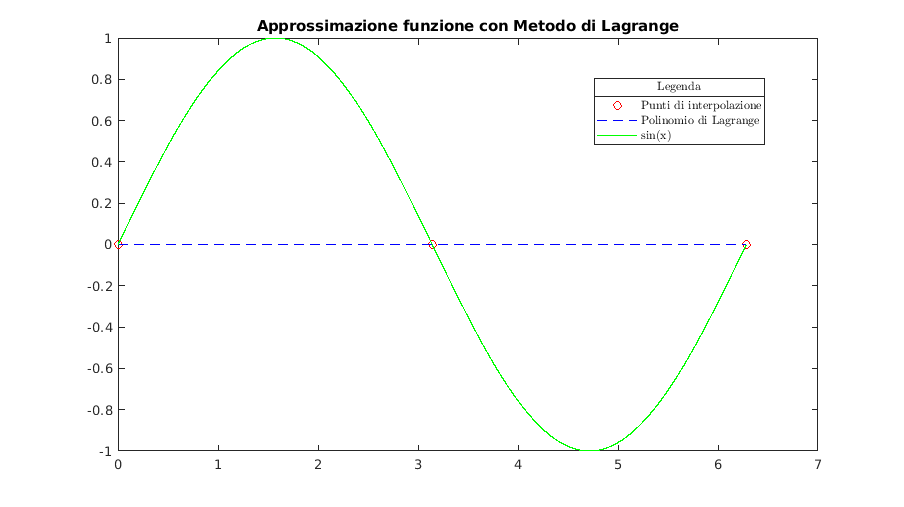
\includegraphics[width=\textwidth]{Grafici/Cap4/es4_lagrange.png}
			Prova
			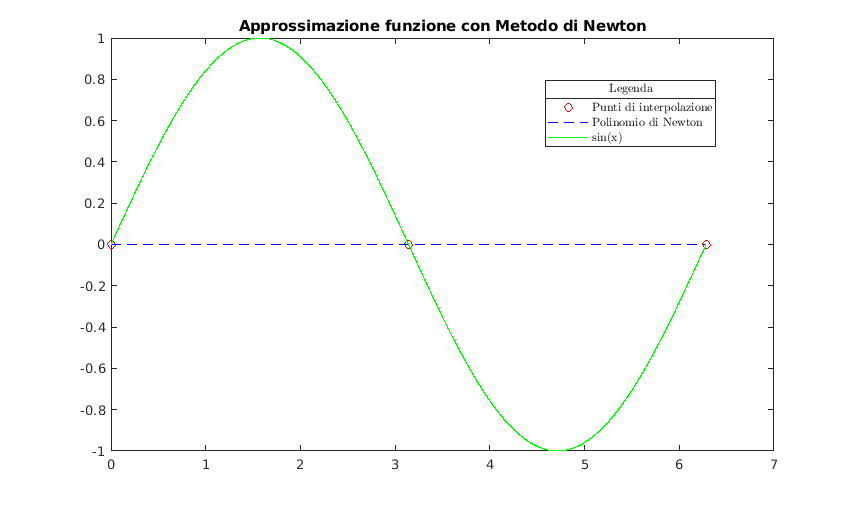
\includegraphics[width=\textwidth]{Grafici/Cap4/es4_newton.png}
			Prova
			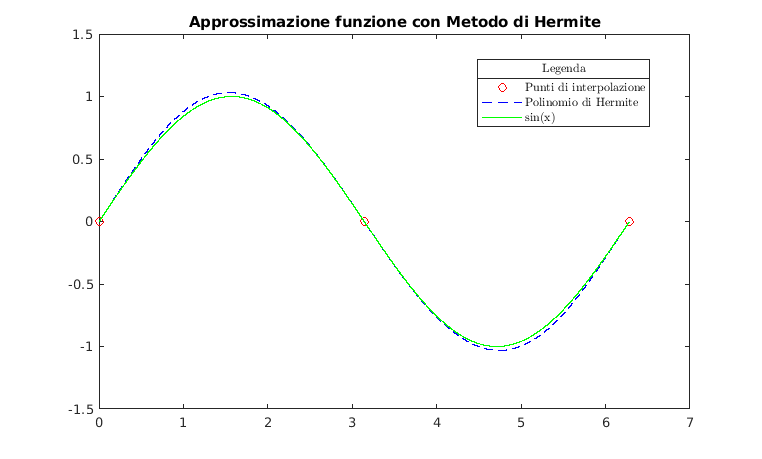
\includegraphics[width=\textwidth]{Grafici/Cap4/es4_hermite.png}
		\section{Esercizio 5}
			Prova
			\lstinputlisting[language = matlab]{CodiciMatlab/Cap4/es5.m}
			Prova
			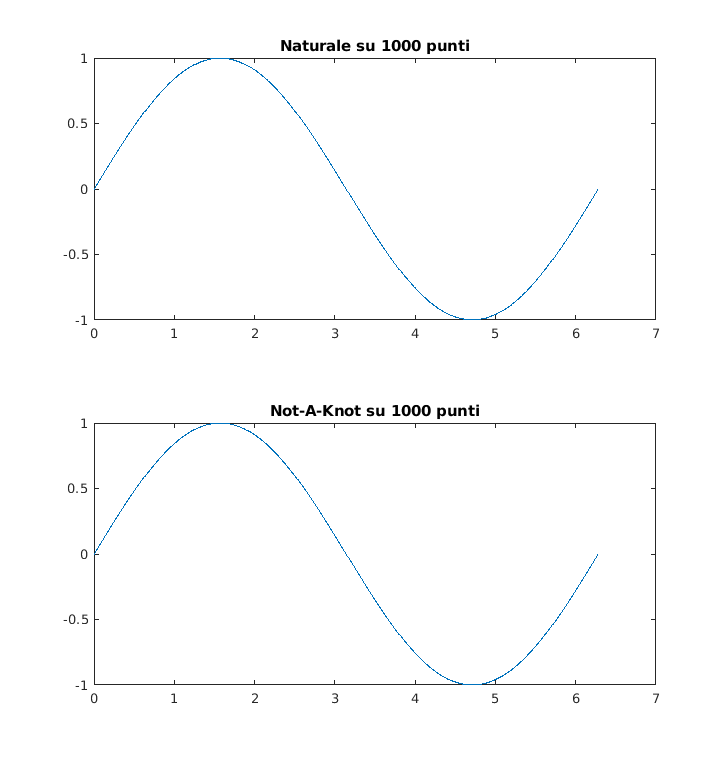
\includegraphics[width=\textwidth]{Grafici/Cap4/es5_spline.png}
		\section{Esercizio 6}
			Prova
			\lstinputlisting[language = matlab]{CodiciMatlab/Cap4/es6.m}
		\section{Esercizio 7}
			Prova
		\section{Esercizio 8}
			Prova
		\section{Esercizio 9}
			Prova
		\section{Esercizio 10}
	
	\chapter{Formule di quadratura}
		\section{Esercizio 1}
			Prova
			\lstinputlisting[language = matlab]{CodiciMatlab/Cap5/es1.m}
		\section{Esercizio 2}
			Prova
			\lstinputlisting[language = matlab]{CodiciMatlab/Cap5/es2.m}
		\section{Esercizio 3}
			Prova
			\lstinputlisting[language = matlab]{CodiciMatlab/Cap5/es3.m}
		\section{Esercizio 4}
			Prova
			\lstinputlisting[language = matlab]{CodiciMatlab/Cap5/es4.m}
		\section{Esercizio 5}
			Prova
			
	\chapter{Calcolo del Google pagerank. Risoluzione iterativa di sistemi lineari}
		\section{Esercizio 1}
			Prova
			\lstinputlisting[language = matlab]{CodiciMatlab/Cap6/es1.m}
		\section{Esercizio 2}
			Prova
			\lstinputlisting[language = matlab]{CodiciMatlab/Cap6/es2.m}
		\section{Esercizio 3}
			Prova
			\lstinputlisting[language = matlab]{CodiciMatlab/Cap6/es3.m}
			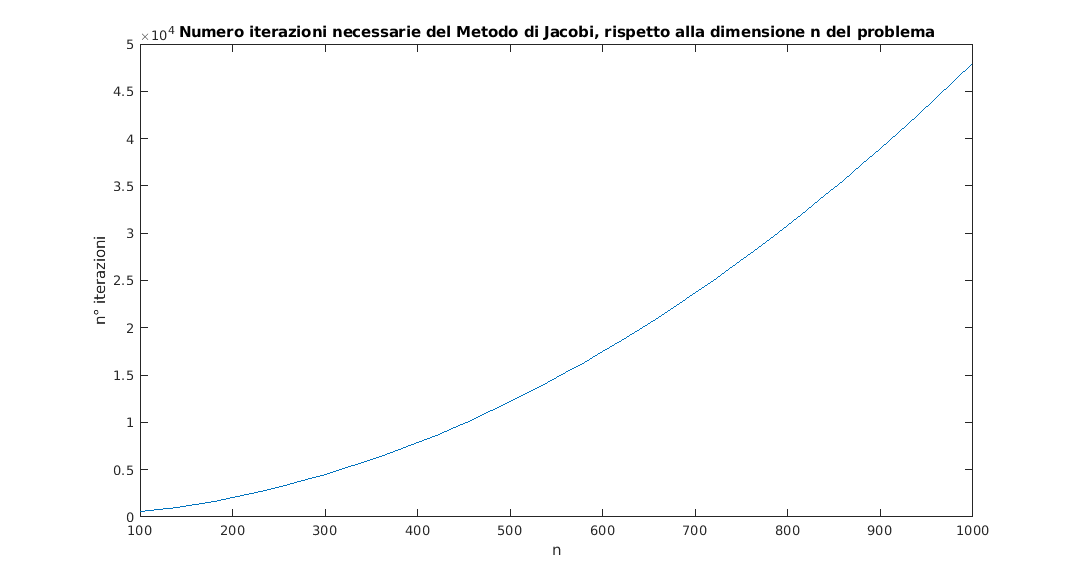
\includegraphics[width=\textwidth]{Grafici/Cap6/es3_jacobi.png}
		\section{Esercizio 4}
			Prova
			\lstinputlisting[language = matlab]{CodiciMatlab/Cap6/es4.m}
			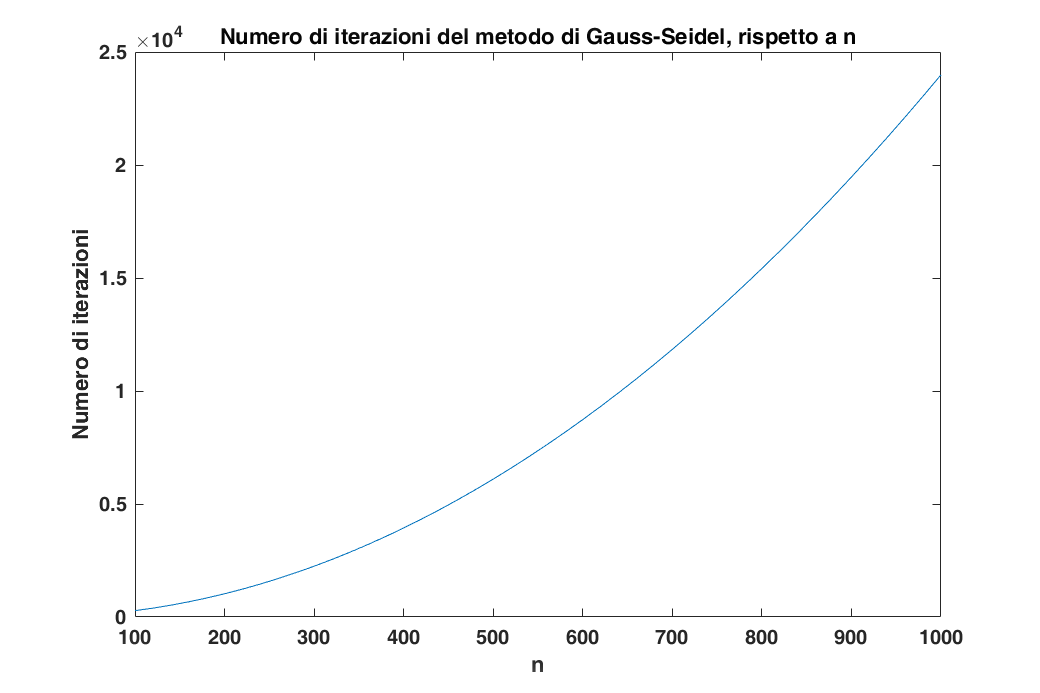
\includegraphics[width=\textwidth]{Grafici/Cap6/es4_gs.png}
		\section{Esercizio 5}
			Prova
			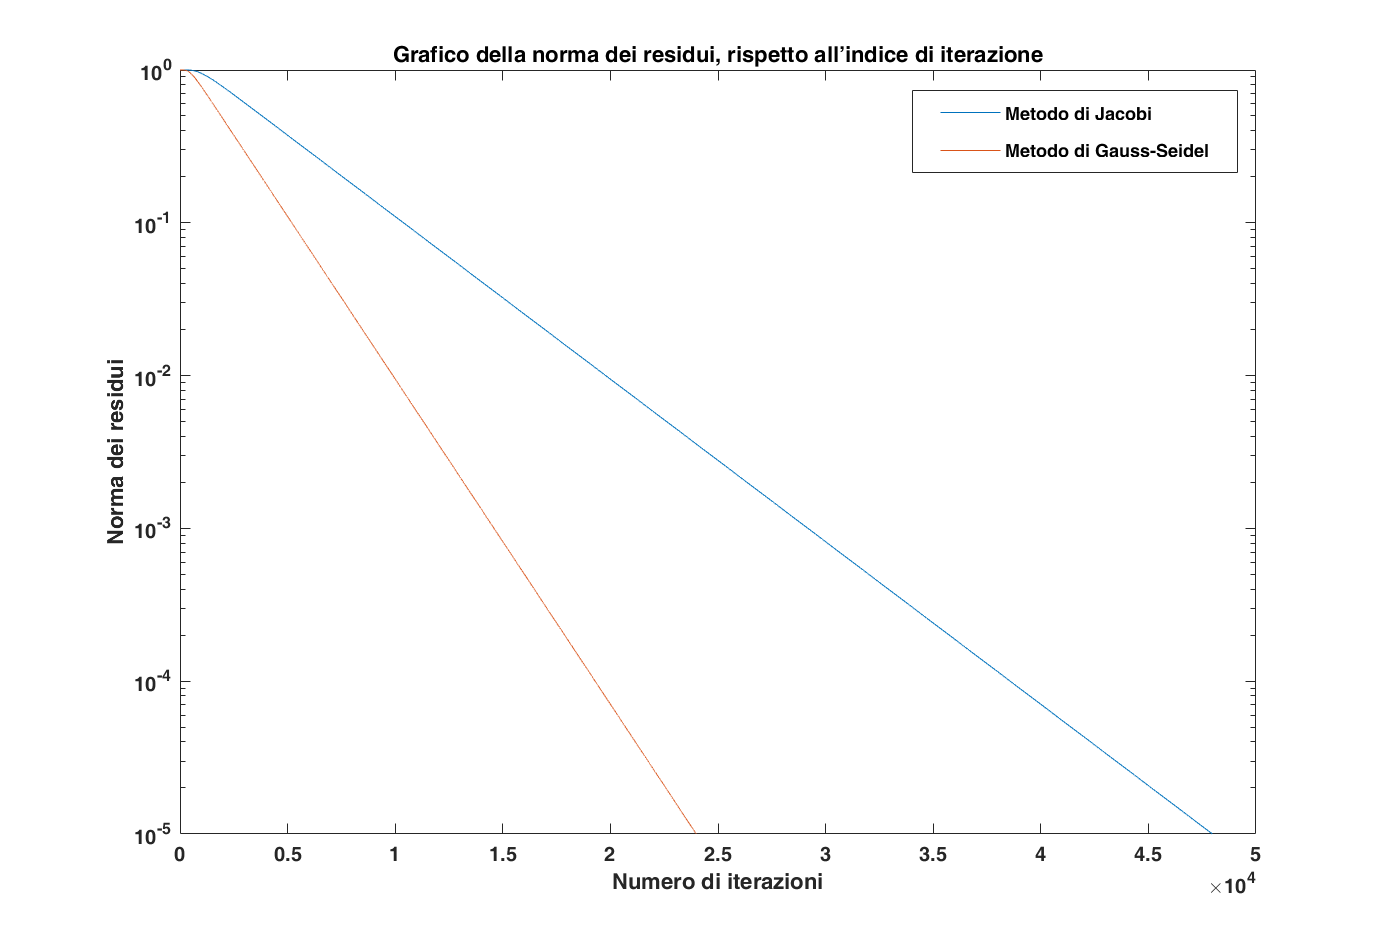
\includegraphics[width=\textwidth]{Grafici/Cap6/es5_normeResidui.png}
				
\end{document}